\documentclass[11pt]{article}
\usepackage[utf8]{inputenc}
\usepackage[T1]{fontenc}
\usepackage[margin=1in]{geometry}
\usepackage{amsmath,amssymb,amsthm}
\usepackage{graphicx}
\usepackage{booktabs}
\usepackage{longtable}
\usepackage{hyperref}
\usepackage{listings}
\usepackage{xcolor}
\hypersetup{colorlinks=true, linkcolor=blue, citecolor=blue, urlcolor=blue}

\lstdefinelanguage{Lean4}{
  morekeywords={theorem,def,noncomputable,import,namespace,end,open,by},
  morecomment=[l]{--},
  morecomment=[s]{/-}{-/},
  sensitive=true,
}
\lstset{basicstyle=\small\ttfamily, language=Lean4, columns=fullflexible, breaklines=true}

% Every number below that comes from this run is a macro generated from
% results/eboss_vs_desi/*.json by scripts/eboss_vs_desi/make_paper_inputs.py.
% generated by scripts/eboss_vs_desi/make_paper_inputs.py -- do not edit
\newcommand{\CambDM}{$2.0\times10^{-4}$}
\newcommand{\CambDV}{$2.9\times10^{-4}$}
\newcommand{\CambH}{$4.8\times10^{-4}$}
\newcommand{\CambPass}{passed}
\newcommand{\CambRd}{147.1027}
\newcommand{\DesiAcc}{0.71}
\newcommand{\DesiCorr}{-0.926}
\newcommand{\DesiDof}{11}
\newcommand{\DesiEmGridDiff}{0.020}
\newcommand{\DesiGridHrd}{101.52}
\newcommand{\DesiGridHrdErr}{0.74}
\newcommand{\DesiGridOm}{0.2978}
\newcommand{\DesiGridOmErr}{0.0086}
\newcommand{\DesiHrd}{101.51}
\newcommand{\DesiHrdErr}{0.75}
\newcommand{\DesiLapHrdErr}{0.74}
\newcommand{\DesiLapOmErr}{0.0086}
\newcommand{\DesiMapChi}{10.27}
\newcommand{\DesiMapHrd}{101.54}
\newcommand{\DesiMapOm}{0.2975}
\newcommand{\DesiNdata}{13}
\newcommand{\DesiOm}{0.2980}
\newcommand{\DesiOmErr}{0.0087}
\newcommand{\DesiTauMax}{30.6}
\newcommand{\FitElgMtwo}{0.27}
\newcommand{\FitGenerated}{2026-09-27 17:10:34}
\newcommand{\FitShaShort}{23f0d1d10062ba81}
\newcommand{\GridN}{301}
\newcommand{\IcElgDev}{0.0028}
\newcommand{\IcElgLowL}{0.19}
\newcommand{\IcElgLowX}{14.88}
\newcommand{\IcElgPeak}{18.328}
\newcommand{\IcElgRef}{18.330}
\newcommand{\IcElgW}{1.007}
\newcommand{\IcLaDH}{8.930}
\newcommand{\IcLaDM}{37.60}
\newcommand{\IcLaRefDH}{8.930}
\newcommand{\IcLaRefDM}{37.60}
\newcommand{\IcLaRefRho}{-0.49}
\newcommand{\IcLaRho}{-0.476}
\newcommand{\IcLaWDH}{0.97}
\newcommand{\IcLaWDM}{0.91}
\newcommand{\IcLxDH}{9.082}
\newcommand{\IcLxDM}{37.33}
\newcommand{\IcLxRefDH}{9.080}
\newcommand{\IcLxRefDM}{37.30}
\newcommand{\IcLxRefRho}{-0.43}
\newcommand{\IcLxRho}{-0.441}
\newcommand{\IcLxWDH}{0.84}
\newcommand{\IcLxWDM}{0.97}
\newcommand{\IcMgsDev}{0.0003}
\newcommand{\IcMgsNegDev}{20.4}
\newcommand{\IcMgsNegPeak}{1.039}
\newcommand{\IcMgsPeak}{4.466}
\newcommand{\IcMgsRef}{4.466}
\newcommand{\IcMgsW}{0.941}
\newcommand{\IcPred}{$9.3\times10^{-15}$}
\newcommand{\LeanSha}{560e3b5d8266a2e2}
\newcommand{\LedgerBlock}{0}
\newcommand{\LedgerClaims}{27}
\newcommand{\LedgerFlag}{0}
\newcommand{\LedgerRc}{0}
\newcommand{\Nburn}{1000}
\newcommand{\NcAll}{all rejected}
\newcommand{\NcCov}{23.34}
\newcommand{\NcEdsDesi}{1409.9}
\newcommand{\NcEdsSdss}{$\infty$}
\newcommand{\NcEdsSgs}{376.4}
\newcommand{\NcGuard}{passed}
\newcommand{\NcPermChi}{13.51}
\newcommand{\NcPermRef}{11.52}
\newcommand{\NcProbeAsCoded}{as-coded boolean: rejected}
\newcommand{\NcProbeOk}{probe check passed}
\newcommand{\NcShift}{12.14}
\newcommand{\NcSwap}{5248.7}
\newcommand{\Nstep}{6000}
\newcommand{\Nwalk}{32}
\newcommand{\PcDBiasHrd}{0.086}
\newcommand{\PcDBiasOm}{0.066}
\newcommand{\PcDCovHrd}{0.665}
\newcommand{\PcDCovOm}{0.655}
\newcommand{\PcDEmCov}{0.65/0.60}
\newcommand{\PcDKsChi}{0.073}
\newcommand{\PcN}{200}
\newcommand{\PcPass}{passed}
\newcommand{\PcSBiasHrd}{0.077}
\newcommand{\PcSBiasOm}{0.045}
\newcommand{\PcSCovHrd}{0.675}
\newcommand{\PcSCovOm}{0.695}
\newcommand{\PcSEmCov}{0.75/0.75}
\newcommand{\PcSKsChi}{0.085}
\newcommand{\PcSeed}{20260927}
\newcommand{\PcTGtTwo}{0.030}
\newcommand{\PcTKs}{0.549}
\newcommand{\PcTMed}{0.672}
\newcommand{\PreregSha}{e0eca89f279cfaac}
\newcommand{\PullDesiHrd}{-0.043}
\newcommand{\PullDesiOm}{+0.055}
\newcommand{\PullSdssHrd}{+0.090}
\newcommand{\PullSdssOm}{-0.017}
\newcommand{\SdssAcc}{0.71}
\newcommand{\SdssCorr}{-0.880}
\newcommand{\SdssDof}{12}
\newcommand{\SdssEmGridDiff}{0.014}
\newcommand{\SdssGridHrd}{100.53}
\newcommand{\SdssGridHrdErr}{1.27}
\newcommand{\SdssGridOm}{0.2987}
\newcommand{\SdssGridOmErr}{0.0162}
\newcommand{\SdssHrd}{100.52}
\newcommand{\SdssHrdErr}{1.29}
\newcommand{\SdssLapHrdErr}{1.24}
\newcommand{\SdssLapOmErr}{0.0158}
\newcommand{\SdssMapChi}{11.52}
\newcommand{\SdssMapHrd}{100.58}
\newcommand{\SdssMapOm}{0.2974}
\newcommand{\SdssNdata}{14}
\newcommand{\SdssOm}{0.2987}
\newcommand{\SdssOmErr}{0.0164}
\newcommand{\SdssTauMax}{29.0}
\newcommand{\SgsAcc}{0.71}
\newcommand{\SgsCorr}{-0.876}
\newcommand{\SgsDof}{10}
\newcommand{\SgsEmGridDiff}{0.010}
\newcommand{\SgsGridHrd}{100.52}
\newcommand{\SgsGridHrdErr}{1.27}
\newcommand{\SgsGridOm}{0.2994}
\newcommand{\SgsGridOmErr}{0.0165}
\newcommand{\SgsHrd}{100.52}
\newcommand{\SgsHrdErr}{1.26}
\newcommand{\SgsLapHrdErr}{1.27}
\newcommand{\SgsLapOmErr}{0.0163}
\newcommand{\SgsMapChi}{10.87}
\newcommand{\SgsMapHrd}{100.58}
\newcommand{\SgsMapOm}{0.2980}
\newcommand{\SgsNdata}{12}
\newcommand{\SgsOm}{0.2993}
\newcommand{\SgsOmErr}{0.0165}
\newcommand{\SgsTauMax}{29.3}
\newcommand{\ShiftHrd}{0.004}
\newcommand{\ShiftOm}{0.032}
\newcommand{\TChi}{1.932}
\newcommand{\TGridChi}{1.889}
\newcommand{\TGridNsig}{0.862}
\newcommand{\TGridOneHrd}{0.675}
\newcommand{\TGridOneOm}{0.045}
\newcommand{\TGridPte}{0.389}
\newcommand{\TGsChi}{1.759}
\newcommand{\TGsNsig}{0.815}
\newcommand{\TGsOneHrd}{0.673}
\newcommand{\TGsOneOm}{0.068}
\newcommand{\TGsPte}{0.415}
\newcommand{\TKdeN}{20000}
\newcommand{\TKdeNsig}{0.939}
\newcommand{\TKdePte}{0.348}
\newcommand{\TMapChi}{2.092}
\newcommand{\TMapNsig}{0.932}
\newcommand{\TMapOneHrd}{0.668}
\newcommand{\TMapOneOm}{0.004}
\newcommand{\TMapPte}{0.351}
\newcommand{\TNsig}{0.877}
\newcommand{\TOneHrd}{0.668}
\newcommand{\TOneOm}{0.041}
\newcommand{\TPte}{0.381}
\newcommand{\WithinTol}{true}


\title{Cross-Survey Consistency of BAO under Flat $\Lambda$CDM:\\
SDSS/eBOSS DR16 versus DESI DR2, Fitted Separately,\\
with a Kernel-Verified Tension Statistic}
\author{AutoevolveAI / ANSE Research Pipeline \\
\small Model-produced by an automated Claude Code pipeline \\
\small (the generating model version is not recorded in the result artifacts); \\
\small reviewed only by an automated model referee, not by a person}
\date{September 27, 2026}

\begin{document}
\sloppy
\maketitle

\begin{abstract}
We fit flat-$\Lambda$CDM, BAO-only, to two surveys \emph{separately}: the
completed SDSS/eBOSS DR16 BAO compilation \cite{alam2021}, using its
distributed grid likelihoods, and DESI DR2 BAO \cite{desi2025dr2}. We then
compare the two posteriors in the $(\Omega_m, h r_d)$ plane. SDSS gives
$\Omega_m=\SdssOm\pm\SdssOmErr$ and $h r_d=(\SdssHrd\pm\SdssHrdErr)$~Mpc.
DESI DR2 gives $\Omega_m=\DesiOm\pm\DesiOmErr$ and
$h r_d=(\DesiHrd\pm\DesiHrdErr)$~Mpc. These reproduce the published values
to within $|\mathrm{pull}|\le0.06\sigma$ on the three targets we could check
against primary sources.

The parameter-difference statistic
$\chi^2=\Delta p^\top(C_\mathrm{SDSS}+C_\mathrm{DESI})^{-1}\Delta p$ gives
$\chi^2=\TChi$ for 2 degrees of freedom, a probability to exceed
(PTE) of $\TPte$, and $N_\sigma=\TNsig$. This passes the preregistered
criterion $N_\sigma<2$ and agrees with DESI DR2's qualitative statement
that its BAO are consistent with SDSS. The statistic treats the two surveys
as independent. Their volumes overlap; if the cross-survey covariance $K$
has $K+K^\top$ positive semidefinite, this is a lower bound with respect to
that overlap ($K$ was not estimated).

The analysis choices, pass criteria and controls were preregistered before
any fit. An injected-parameter positive control, run as preregistered on the
SDSS Gaussian-summary variant and on DESI (not on the SDSS baseline grid
likelihood), and the gated negative controls behave as required. In Lean~4 we kernel-verify nine algebraic properties of
the tension statistic, including that it equals Mathlib's
$d\cdot(C^{-1}d)$, is symmetric in the two surveys, and is a
positive-definite quadratic form. All nine report exactly the trusted axioms.
This is a reproduction and consistency exercise. It is not a new
cosmological constraint.
\end{abstract}

\section{Introduction}

BAO surveys measure the transverse comoving distance $D_M(z)/r_d$, the Hubble
distance $D_H(z)/r_d=c/(H(z)r_d)$, and the isotropic combination
$D_V(z)/r_d=[z D_M^2 D_H]^{1/3}/r_d$. In flat $\Lambda$CDM,
$E(z)=\sqrt{\Omega_m(1+z)^3+1-\Omega_m}$, and BAO-only data constrain exactly
two parameters, $\Omega_m$ and $h r_d$. DESI DR2 states that it samples
these two parameters when fitting BAO alone \cite{desi2025dr2}.

DESI DR2 says its BAO results are ``consistent with DESI DR1 and SDSS''. In
a four-bin comparison it concludes ``there is no significant discrepancy''
(largest differences $1.49\sigma$ in $\alpha_\mathrm{iso}$ and $1.69\sigma$
in $\alpha_\mathrm{AP}$), and it gives the LRG2 $D_M/r_d$ difference against
eBOSS as $1.5\sigma$ to $2.6\sigma$ \cite{desi2025dr2}. It publishes no
tension number for SDSS versus DR2 in the $(\Omega_m,h r_d)$ plane. The DR1
analysis defines a parameter-difference statistic, its eq.~(4.2), which it
applies to the comparison of DESI DR1 BAO with the CMB (\S4.1);
its comparison of DR1 with SDSS (\S3.3) is qualitative only, reporting ``no
significant difference in $\Omega_m$ and a shift of just $\sim1\sigma$ in
$r_d h$'' \cite{desi2024vi}. This paper computes the eq.~(4.2) number for
SDSS versus DR2 from the
public data products, fitting the two surveys separately and never
combining them.

The exercise follows an earlier flat-$\Lambda$CDM reproduction of DESI DR1
in the same repository (\texttt{papers/bao\_flcdm/}), which matched DESI's
published values to within $0.07\sigma$ and $0.11\sigma$. It adds three
things: non-Gaussian grid likelihoods, a preregistration fixed before any
fit, and a formalization of the comparison statistic itself.

\section{Data}

All input files come from a local copy of a BAO data collection. Its
README lists the DESI DR2 and DR1 files, and the eBOSS DR16, SDSS DR7 MGS
and SDSS DR12 files ``as originally distributed with CosmoMC''. The
likelihood conventions (redshifts, table formats, the MGS
$\alpha$ rescaling) were read from the Cobaya source \cite{cobaya}. Each
file's SHA-256 was fixed in the preregistration and re-verified by the fit
(\texttt{input\_sha256\_verified: true}).

\paragraph{SDSS/eBOSS DR16 \cite{alam2021}.} The baseline likelihood is the
sum of the pieces below, with no covariance between samples, as in
\cite{alam2021}:
\begin{itemize}
\item MGS ($z=0.15$): a $\chi^2(\alpha)$ table, with
  $\alpha=(D_V/r_d)/4.29720761315$.
\item Gaussian pieces (Table~\ref{tab:sdss}): BOSS DR12 galaxies at $z=0.38$
  and $0.51$, eBOSS LRG at $z=0.698$, and eBOSS QSO at $z=1.48$, with the
  distributed covariances.
\item eBOSS ELG ($z=0.845$): a 1D likelihood table in $D_V/r_d$.
\item Ly$\alpha$ auto and Ly$\alpha\times$QSO ($z=2.334$): two 2D
  likelihood grids in $(D_M/r_d, D_H/r_d)$, interpolated in $\ln L$ with
  bicubic splines and an explicit bounds check.
\end{itemize}

Three sets of files were excluded before any fit:
\begin{itemize}
\item the DESI DR1 + eBOSS combined Ly$\alpha$ file, because it contains
  DESI data. The SDSS likelihood reads only a fixed dictionary of SDSS
  filenames whose SHA-256 hashes are preregistered; a code guard checks the
  filename, the allow-list and the hash, and raises otherwise
  (Section~\ref{sec:controls});
\item the DR12 consensus file, whose $z=0.61$ bin double-counts the eBOSS
  LRG volume;
\item all files that include RSD or full-shape information.
\end{itemize}

A \emph{Gaussian-summary} variant serves as a sensitivity check and as the
basis of the positive control. It replaces MGS and ELG with the Table~III
values of \cite{alam2021}, and replaces the two Ly$\alpha$ grids with the
joint auto+cross result of \cite{dmdb2020}, eq.~(43).

\begin{table}[h]
\centering
\caption{Gaussian pieces of the SDSS likelihood, read from the distributed
files. $\sigma=\sqrt{\mathrm{diag}\,C}$. The DR12 file gives
$\sigma(D_H,0.38)=0.729$, while \cite{alam2021} Table~III rounds it to
0.76. The file is used, and this difference was recorded before the fit.}
\label{tab:sdss}
\begin{tabular}{lcccc}
\toprule
Sample & $z$ & Quantity & Value & $\sigma$ \\
\midrule
\csname @@input\endcsname gen_sdss_table.tex
\bottomrule
\end{tabular}
\end{table}

\paragraph{DESI DR2 \cite{desi2025dr2}.} The data are
\texttt{desi\_gaussian\_bao\_ALL\_GCcomb\_\{mean,cov\}.txt}: 13 data points
with a $13\times13$ covariance (Table~\ref{tab:desi}).

\begin{table}[h]
\centering
\caption{DESI DR2 BAO data vector as distributed. $\sigma=\sqrt{\mathrm{diag}\,C}$.
The fit uses the full covariance.}
\label{tab:desi}
\begin{tabular}{lcccc}
\toprule
Survey & $z$ & Quantity & Value & $\sigma$ \\
\midrule
\csname @@input\endcsname gen_desi_table.tex
\bottomrule
\end{tabular}
\end{table}

\section{Method}

The predictions are $D_M/r_d=(c/100\,h r_d)\int_0^z dz'/E(z')$,
$D_H/r_d=c/(100\,h r_d\,E(z))$ and the $D_V$ combination above. Radiation is
neglected. Section~\ref{sec:camb} checks this against CAMB. Three prediction
codes are required to agree to $10^{-4}$ relative: astropy
\texttt{FlatLambdaCDM}, \texttt{scipy.integrate.quad}, and Gauss--Legendre
quadrature. Their measured maximum disagreement was \IcPred.

The priors are flat, with $\Omega_m\in[0.05,0.95]$ and
$h r_d\in[60,150]$~Mpc. Each dataset is sampled with \texttt{emcee}
(\Nwalk\ walkers, \Nstep\ steps, burn-in \Nburn). Every chain satisfies
$50\,\tau<\Nstep$, with a maximum autocorrelation time $\tau$ of
\DesiTauMax\ for DESI and \SdssTauMax\ for SDSS. We report the posterior
mean $\pm$ standard deviation, which is the DESI convention.

There are two independent cross-checks:
\begin{itemize}
\item a normalized $\GridN\times\GridN$ grid posterior; its means agree with
  emcee within \SdssEmGridDiff$\sigma$ for SDSS and \DesiEmGridDiff$\sigma$
  for DESI;
\item a MAP estimate with Laplace errors.
\end{itemize}

\paragraph{Tension statistic.} With $p=(\Omega_m, h r_d)$, the statistic is
$\chi^2=\Delta p^\top(C_\mathrm{SDSS}+C_\mathrm{DESI})^{-1}\Delta p$. This is
eq.~(18) of \cite{desi2025dr2} and eq.~(4.2) of \cite{desi2024vi}. It is
converted to a PTE for 2 degrees of freedom and then to a two-sided Gaussian
$N_\sigma$. The code is \texttt{bao\_lib.tension}. We also report the 1D
parameter differences and a KDE parameter-shift PTE on the chains, which
does not assume Gaussian posteriors.

\section{Preregistration}

\texttt{results/eboss\_vs\_desi/preregistration.json} (SHA-256 prefix
\texttt{\PreregSha}) was written at 2026-09-27T15:50Z and amended once,
before any fit. The fit output records that hash, and it was unchanged at
the time of the fit. The preregistration fixed the following:
\begin{itemize}
\item \textbf{Targets.}
  \begin{itemize}
  \item SDSS $\Omega_m=0.299\pm0.016$, from Table~IV of \cite{alam2021}:
    $\Omega_\mathrm{DE}=0.701^{+0.017}_{-0.015}$.
  \item DESI DR2 $\Omega_m=0.2975\pm0.0086$ and
    $h r_d=(101.54\pm0.73)$~Mpc, from eq.~(17) of \cite{desi2025dr2}.
  \item SDSS $h r_d=(100.4\pm1.3)$~Mpc. This is quoted by \cite{desi2024vi}
    \S4.1, which cites \cite{alam2021}, but it was not found in the fetched
    pages of \cite{alam2021}. It is therefore reported but not counted.
  \end{itemize}
\item \textbf{Tolerance.} $|\mathrm{pull}|<0.5\sigma$ on the three
  primary-verified targets.
\item \textbf{Consistency criterion.} $N_\sigma<2$.
\item \textbf{Expected range.} From the published means alone, $N_\sigma$
  falls between 0.32 and 1.56 as the unpublished SDSS
  $\Omega_m$--$h r_d$ correlation is scanned over $[-0.95,0.95]$. This range
  is an expectation, not a criterion.
\item \textbf{Controls.} All controls and their thresholds
  (Section~\ref{sec:controls}).
\end{itemize}

\section{Controls}\label{sec:controls}

\paragraph{Instrument check on the grid likelihoods} (no cosmology). Each
interpolated table must reproduce its published peak and width:
\begin{itemize}
\item MGS: peak \IcMgsPeak\ versus \IcMgsRef, which is
  \IcMgsDev$\sigma$ off; width ratio \IcMgsW.
\item ELG: peak \IcElgPeak\ versus \IcElgRef; width ratio \IcElgW. The
  distributed table is truncated at its lower edge, $D_V/r_d=\IcElgLowX$,
  where $L/L_\mathrm{max}$ is still \IcElgLowL; below that edge our
  likelihood returns $-\infty$ in $\ln L$. This does not affect the real fit:
  the ELG term contributes \FitElgMtwo\ to $-2\ln L$ at the SDSS MAP.
\item Ly$\alpha$ auto: peak $(D_M,D_H)=(\IcLaDM,\IcLaDH)$ versus
  $(\IcLaRefDM,\IcLaRefDH)$; $\rho=\IcLaRho$ versus $\IcLaRefRho$; width
  ratios \IcLaWDM/\IcLaWDH.
\item Ly$\alpha\times$QSO: peak $(\IcLxDM,\IcLxDH)$ versus
  $(\IcLxRefDM,\IcLxRefDH)$; $\rho=\IcLxRho$ versus $\IcLxRefRho$; width
  ratios \IcLxWDM/\IcLxWDH. The preregistered width tolerance for
  Ly$\alpha$ is 0.25.
\item Paired negative: dropping the MGS $\alpha$ rescaling must fail. It
  does, with a peak at \IcMgsNegPeak, \IcMgsNegDev$\sigma$ off.
\end{itemize}

\paragraph{Positive control} (\PcPass). There were \PcN\ realizations of
synthetic Gaussian data, injected at $(0.2975, 101.54)$ with seed \PcSeed.
The preregistered thresholds are 1$\sigma$ coverage in $[0.60,0.76]$ and
$|\mathrm{bias}|<0.2\sigma$.
\begin{itemize}
\item SDSS Gaussian-summary: coverage \PcSCovOm\ for $\Omega_m$ and
  \PcSCovHrd\ for $h r_d$; bias \PcSBiasOm$\sigma$ and \PcSBiasHrd$\sigma$.
\item DESI DR2: coverage \PcDCovOm\ and \PcDCovHrd; bias \PcDBiasOm$\sigma$
  and \PcDBiasHrd$\sigma$.
\item Tension calibration on pairs drawn from the same parameters: median
  $N_\sigma=\PcTMed$; KS test of the PTE against a uniform distribution,
  $p=\PcTKs$; fraction with $N_\sigma>2$ equal to \PcTGtTwo.
\item emcee subset of 20 realizations: coverage \PcSEmCov\ for SDSS and
  \PcDEmCov\ for DESI.
\item Not gated, reported for completeness: a KS test of the injected
  realizations' $\chi^2_\mathrm{min}$ against $\chi^2(\mathrm{dof})$ gives
  $p=\PcSKsChi$ (SDSS Gaussian-summary) and $p=\PcDKsChi$ (DESI DR2), so
  the fit-quality distribution is only marginally consistent with the
  nominal one.
\end{itemize}
This control never exercises the SDSS baseline grid likelihood (MGS, ELG
and Ly$\alpha$ tables). It runs on the Gaussian-summary variant only, as
preregistered. For the baseline, the evidence is indirect: the instrument
check below reproduces every table's published peak and width, and the
baseline and variant posteriors differ by \ShiftOm$\sigma$ in $\Omega_m$ and
\ShiftHrd$\sigma$ in $h r_d$.

\paragraph{Negative controls} (\NcAll).
\begin{itemize}
\item No-$\Lambda$ model (Einstein--de Sitter) on DESI:
  $\Delta(-2\ln L)=\NcEdsDesi$, against a required $>25$. On the SDSS
  baseline the value is \NcEdsSdss. The preregistered boolean passes, but
  only \emph{by construction}: $\Omega_m=1$ predictions fall outside the grid
  tables for every $h r_d$, so the test does not discriminate. A probe
  likelihood that returns $+\infty$ everywhere passes the as-coded boolean
  too (\NcProbeAsCoded). A stricter gate was therefore added on top of
  the preregistered one (recorded as such in
  \texttt{negative\_controls.json}): it also requires both minima to be
  finite, and the SDSS EdS test is gated on the Gaussian-summary variant,
  $\Delta=\NcEdsSgs$. Under the stricter gate the SDSS baseline is recorded
  as non-discriminating and the $+\infty$ probe is correctly not rejected
  (\NcProbeOk).
\item DESI $D_M\leftrightarrow D_H$ swap: $\chi^2/\mathrm{dof}=\NcSwap$,
  against a required $>3$.
\item DESI covariance divided by 25: $\chi^2/\mathrm{dof}=\NcCov$, against a
  required $>3$.
\item Every DESI ratio multiplied by 0.93: $N_\sigma=\NcShift$ against SDSS.
  The requirement was $>3$, and the closed-form expectation was at least
  5.44.
\item Combination guard (\NcGuard): it raised on the excluded DESI+eBOSS
  Ly$\alpha$ file (filename check), on a copy of the DESI DR2 mean file under
  a non-DESI name (allow-list check), and on the same copy renamed to a real
  SDSS filename (SHA-256 check); all ten real SDSS files were accepted. The
  guard is a
  safeguard against wiring mistakes, not a proof that no DESI information
  enters the SDSS files.
\item Report-only permutation of the SDSS covariance:
  $-2\ln L_\mathrm{min}=\NcPermChi$, versus \NcPermRef\ unpermuted.
\end{itemize}

\paragraph{CAMB background cross-check}\label{sec:camb} (\CambPass). CAMB
2.0.4 was run at three parameter points. The largest relative differences
between the analytic model and CAMB at the data redshifts are \CambDM\ in
$D_M$, \CambH\ in $H$ and \CambDV\ in $D_V$, all below the $10^{-3}$ gate.
At the Planck-2018 point, CAMB gives $r_\mathrm{drag}=\CambRd$~Mpc.

\section{Results}

\begin{table}[h]
\centering
\caption{Flat-$\Lambda$CDM BAO-only posteriors, each survey fitted
separately. The primary estimate is the emcee mean $\pm$ standard deviation.
Pulls are measured against the published values and use the published
$\sigma$. $\dagger$: secondary-sourced target, not counted toward the
tolerance.}
\label{tab:results}
\small
\setlength{\tabcolsep}{4pt}
\begin{tabular}{lcccc}
\toprule
Dataset & $\Omega_m$ & $h r_d$ [Mpc] & corr & $-2\ln L_\mathrm{min}$ (dof) \\
\midrule
SDSS/eBOSS DR16 (baseline, emcee) & $\SdssOm\pm\SdssOmErr$ & $\SdssHrd\pm\SdssHrdErr$ & $\SdssCorr$ & \SdssMapChi\ (\SdssDof, nominal) \\
\quad grid & $\SdssGridOm\pm\SdssGridOmErr$ & $\SdssGridHrd\pm\SdssGridHrdErr$ & & \\
\quad MAP (Laplace $\sigma$) & $\SdssMapOm\pm\SdssLapOmErr$ & $\SdssMapHrd\pm\SdssLapHrdErr$ & & \\
SDSS Gaussian-summary variant & $\SgsOm\pm\SgsOmErr$ & $\SgsHrd\pm\SgsHrdErr$ & $\SgsCorr$ & \SgsMapChi\ (\SgsDof) \\
DESI DR2 (emcee) & $\DesiOm\pm\DesiOmErr$ & $\DesiHrd\pm\DesiHrdErr$ & $\DesiCorr$ & \DesiMapChi\ (\DesiDof) \\
\quad grid & $\DesiGridOm\pm\DesiGridOmErr$ & $\DesiGridHrd\pm\DesiGridHrdErr$ & & \\
\quad MAP (Laplace $\sigma$) & $\DesiMapOm\pm\DesiLapOmErr$ & $\DesiMapHrd\pm\DesiLapHrdErr$ & & \\
\midrule
Published SDSS \cite{alam2021,desi2024vi} & $0.299\pm0.016$ & $100.4\pm1.3^\dagger$ & & \\
Published DESI DR2 \cite{desi2025dr2} & $0.2975\pm0.0086$ & $101.54\pm0.73$ & $-0.92$ & 10.2 (11) \\
\midrule
Pull SDSS & $\PullSdssOm\sigma$ & $\PullSdssHrd\sigma^\dagger$ & & \\
Pull DESI DR2 & $\PullDesiOm\sigma$ & $\PullDesiHrd\sigma$ & & \\
\bottomrule
\end{tabular}
\end{table}

\begin{table}[h]
\centering
\caption{SDSS versus DESI DR2 parameter-difference statistic (2 dof,
surveys treated as independent).}
\label{tab:tension}
\begin{tabular}{lccccc}
\toprule
Estimator & $\chi^2$ & PTE & $N_\sigma$ & 1D $\Omega_m$ & 1D $h r_d$ \\
\midrule
emcee moments (primary) & \TChi & \TPte & \textbf{\TNsig} & \TOneOm$\sigma$ & \TOneHrd$\sigma$ \\
grid moments & \TGridChi & \TGridPte & \TGridNsig & \TGridOneOm$\sigma$ & \TGridOneHrd$\sigma$ \\
MAP + Laplace & \TMapChi & \TMapPte & \TMapNsig & \TMapOneOm$\sigma$ & \TMapOneHrd$\sigma$ \\
Gaussian-summary SDSS & \TGsChi & \TGsPte & \TGsNsig & \TGsOneOm$\sigma$ & \TGsOneHrd$\sigma$ \\
KDE parameter shift (\TKdeN\ samples) & -- & \TKdePte & \TKdeNsig & -- & -- \\
\bottomrule
\end{tabular}
\end{table}

\begin{figure}[h]
\centering
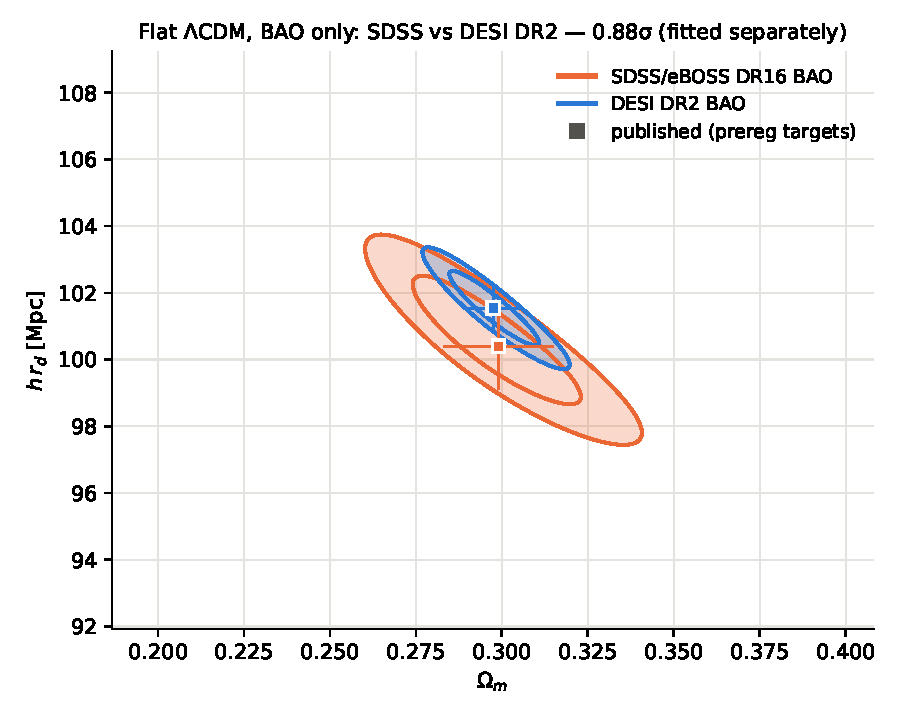
\includegraphics[width=0.75\textwidth]{../../results/eboss_vs_desi/eboss_vs_desi_contours.pdf}
\caption{68.3\% and 95.4\% highest-density contours of the normalized grid
posteriors, with SDSS/eBOSS DR16 in orange and DESI DR2 in blue. The squares
with error bars are the preregistered published targets.}
\label{fig:contours}
\end{figure}

All three primary-verified targets are reproduced within tolerance
(\texttt{within\_tolerance} = \WithinTol). The SDSS baseline and the
Gaussian-summary variant differ by only \ShiftOm$\sigma$ in $\Omega_m$ and
\ShiftHrd$\sigma$ in $h r_d$. The non-Gaussian grid likelihoods therefore do
not drive the result.

The five tension estimators range from \TGsNsig\ to \TKdeNsig$\sigma$. The
primary value, $N_\sigma=\TNsig$, satisfies the preregistered $N_\sigma<2$.
Most of the difference lies in $h r_d$ (\TOneHrd$\sigma$ in 1D). The
$\Omega_m$ values agree closely (\TOneOm$\sigma$). The measured SDSS
correlation, $\SdssCorr$, puts the result inside the preregistered expected
range, between the values for correlations $-0.8$ (0.74$\sigma$) and $-0.9$
(1.10$\sigma$).

\section{Lean 4 formalization of the tension statistic}

\texttt{formal/ANSE/BAO\_Consistency.lean} (SHA-256 prefix
\texttt{\LeanSha}, namespace \texttt{ANSE.BAOConsistency}) formalizes the
statistic that \texttt{bao\_lib.tension} evaluates: \texttt{dp = p1 - p2},
\texttt{C = c1 + c2}, \texttt{chi2 = dp @ solve(C, dp)}. The definitions are:
\begin{gather*}
\texttt{tension1D}\,\mu_1\,\sigma_1\,\mu_2\,\sigma_2=\frac{(\mu_1-\mu_2)^2}{\sigma_1^2+\sigma_2^2},\\
\texttt{chi2}\,a\,b\,c\,d_1\,d_2=\frac{c d_1^2-2 b d_1 d_2+a d_2^2}{ac-b^2},
\end{gather*}
and \texttt{surveyTension} is \texttt{chi2} applied to $C_S+C_D$ and
$p_S-p_D$. The imports are pinned to the locally built Mathlib subset, with
no \texttt{import Mathlib}. The toolchain is
\texttt{leanprover/lean4:v4.34.0-rc2}.

The theorem statements are extracted verbatim from the source by
\texttt{make\_paper\_inputs.py}. Proofs are elided, and the Unicode glyphs
are typeset as math symbols ($\cdot_v$ is Mathlib's \texttt{dotProduct} and
$*_v$ is \texttt{mulVec}):
\begin{lstlisting}[mathescape]
theorem tension1D_symm ($\mu$1 $\sigma$1 $\mu$2 $\sigma$2 : $\mathbb{R}$) :
    tension1D $\mu$1 $\sigma$1 $\mu$2 $\sigma$2 = tension1D $\mu$2 $\sigma$2 $\mu$1 $\sigma$1 := ...

theorem tension1D_nonneg ($\mu$1 $\sigma$1 $\mu$2 $\sigma$2 : $\mathbb{R}$) : 0 $\le$ tension1D $\mu$1 $\sigma$1 $\mu$2 $\sigma$2 := ...

theorem tension1D_eq_zero_iff {$\mu$1 $\sigma$1 $\mu$2 $\sigma$2 : $\mathbb{R}$} (h$\sigma$ : 0 < $\sigma$1) :
    tension1D $\mu$1 $\sigma$1 $\mu$2 $\sigma$2 = 0 $\leftrightarrow$ $\mu$1 = $\mu$2 := ...

theorem chi2_eq_dotProduct_inv_mulVec (a b c d1 d2 : $\mathbb{R}$) (hdet : a * c - b ^ 2 $\neq$ 0) :
    ![d1, d2] $\cdot_v$ ((!![a, b; b, c])$^{-1}$ $*_v$ ![d1, d2]) = chi2 a b c d1 d2 := ...

theorem chi2_nonneg {a b c : $\mathbb{R}$} (ha : 0 < a) (hdet : 0 < a * c - b ^ 2) (d1 d2 : $\mathbb{R}$) :
    0 $\le$ chi2 a b c d1 d2 := ...

theorem chi2_eq_zero_iff {a b c : $\mathbb{R}$} (ha : 0 < a) (hdet : 0 < a * c - b ^ 2) (d1 d2 : $\mathbb{R}$) :
    chi2 a b c d1 d2 = 0 $\leftrightarrow$ d1 = 0 $\wedge$ d2 = 0 := ...

theorem surveyTension_symm (mS1 mS2 aS bS cS mD1 mD2 aD bD cD : $\mathbb{R}$) :
    surveyTension mS1 mS2 aS bS cS mD1 mD2 aD bD cD
      = surveyTension mD1 mD2 aD bD cD mS1 mS2 aS bS cS := ...

theorem posdef_add {aS bS cS aD bD cD : $\mathbb{R}$}
    (haS : 0 < aS) (hdS : 0 < aS * cS - bS ^ 2)
    (haD : 0 < aD) (hdD : 0 < aD * cD - bD ^ 2) :
    0 < aS + aD $\wedge$ 0 < (aS + aD) * (cS + cD) - (bS + bD) ^ 2 := ...

theorem surveyTension_nonneg_and_zero_iff {mS1 mS2 aS bS cS mD1 mD2 aD bD cD : $\mathbb{R}$}
    (haS : 0 < aS) (hdS : 0 < aS * cS - bS ^ 2)
    (haD : 0 < aD) (hdD : 0 < aD * cD - bD ^ 2) :
    0 $\le$ surveyTension mS1 mS2 aS bS cS mD1 mD2 aD bD cD $\wedge$
      (surveyTension mS1 mS2 aS bS cS mD1 mD2 aD bD cD = 0 $\leftrightarrow$ mS1 = mD1 $\wedge$ mS2 = mD2) := ...
\end{lstlisting}


The file was compiled with \texttt{lake env lean} in the round-2 fix stage
of this pipeline, after its last edit (a docstring rewording on
\texttt{tension1D\_eq\_zero\_iff}; source sha256 prefix \LeanSha), and exited
with code 0, with no errors, no warnings and no \texttt{sorry}. The file's own \texttt{\#print axioms} lines produced the
output below. It is verbatim except that each line is wrapped after the
theorem name, and the final \texttt{rc=0} line is the exit code, appended by
the shell:
\begin{verbatim}
'ANSE.BAOConsistency.tension1D_symm'
    depends on axioms: [propext, Classical.choice, Quot.sound]
'ANSE.BAOConsistency.tension1D_nonneg'
    depends on axioms: [propext, Classical.choice, Quot.sound]
'ANSE.BAOConsistency.tension1D_eq_zero_iff'
    depends on axioms: [propext, Classical.choice, Quot.sound]
'ANSE.BAOConsistency.chi2_eq_dotProduct_inv_mulVec'
    depends on axioms: [propext, Classical.choice, Quot.sound]
'ANSE.BAOConsistency.chi2_nonneg'
    depends on axioms: [propext, Classical.choice, Quot.sound]
'ANSE.BAOConsistency.chi2_eq_zero_iff'
    depends on axioms: [propext, Classical.choice, Quot.sound]
'ANSE.BAOConsistency.surveyTension_symm'
    depends on axioms: [propext, Classical.choice, Quot.sound]
'ANSE.BAOConsistency.posdef_add'
    depends on axioms: [propext, Classical.choice, Quot.sound]
'ANSE.BAOConsistency.surveyTension_nonneg_and_zero_iff'
    depends on axioms: [propext, Classical.choice, Quot.sound]
rc=0
\end{verbatim}


Every footprint is exactly the trusted set
$\{\texttt{propext},\texttt{Classical.choice},\texttt{Quot.sound}\}$. The
\textsc{SocrateAI-Scientific-Elenchus} scanner (\texttt{elenchus\_check.py})
reported ``no findings''.

\paragraph{What the Lean results do and do not say.} The Lean results are
exact facts about the statistic:
\begin{itemize}
\item the closed-form \texttt{chi2} equals Mathlib's matrix expression, so
  it is not an ad hoc formula;
\item the statistic is symmetric under swapping SDSS and DESI;
\item it is non-negative, and zero exactly when the two means coincide,
  whenever both posterior covariances are positive definite;
\item the matrix inverted by the fit is positive definite whenever both
  inputs are (\texttt{posdef\_add}).
\end{itemize}
The file asserts nothing numeric. The values $\chi^2=\TChi$ and
$N_\sigma=\TNsig$ are not kernel-checked, and neither is the conversion from
PTE to $N_\sigma$. The match between the Lean definitions and the Python
code is a reading of both, not a kernel fact. In the claim ledger it is
filed at Tier~C (Section~\ref{sec:ledger}).

\section{Claim ledger}\label{sec:ledger}

The claims are registered in Elenchus's tier-capped ledger format in
\texttt{results/eboss\_vs\_desi/ledger/}. There are \LedgerClaims\ claims,
each with a content-addressed evidence blob:
\begin{itemize}
\item 9 at Tier A: the Lean axiom footprints (statement audit by an
  automated model referee, not a person);
\item 8 at Tier B: the harness outputs;
\item 8 at Tier L: the citations, and every comparison with a published
  number;
\item 2 at Tier C: the lower-bound argument, and the claim that the Lean
  definitions match the code.
\end{itemize}

The gate (\texttt{tools/ledger.py -{}-evidence-dir}) reports \LedgerBlock\
block findings and \LedgerFlag\ flags, and exits with code \LedgerRc.

That exit code needs a caveat about who did the audit. Before the fix
round, every Tier~A row had \texttt{audit: null}. The gate then raised one
\texttt{LEDGER\_UNAUDITED\_TIER\_A} flag per row and exited with code~1. In
the round-2 fix stage, the Lean statement audit of the round-2 referee
(\texttt{results/eboss\_vs\_desi/referee\_report\_round2.json}) was
recorded on the ledger rows. That referee judged all nine statements
faithful to the code. \emph{It is an automated model referee, not a person.}
Each audit object says so (\texttt{auditor\_is\_person: false},
\texttt{human\_audit: "open"}). Elenchus's own design treats this audit as a
person's act. Exit code~\LedgerRc\ therefore means that a model referee
judged the statements faithful. No human statement audit has happened yet.

The referee audited the source before the docstring rewording it asked for.
The ledger builder checks that the saved diff between the two versions
touches no declaration or proof line before it carries the audit over.

Four hand-built mutations of the ledger are each caught. Three produce a
block finding: refiling a comparison-with-published claim at Tier~B
(\texttt{LEDGER\_TIER\_INVERSION}), changing one byte of an evidence blob
(\texttt{LEDGER\_EVIDENCE\_MISMATCH}), and refiling a citation at Tier~A
(\texttt{LEDGER\_KIND\_OVERCLAIM}). The fourth, removing one Tier~A audit
object, brings back the \texttt{LEDGER\_UNAUDITED\_TIER\_A} flag and
exit~1. The gate therefore discriminates on this ledger's content, and the
exit~0 depends on the recorded audits.

\section{Deviations from the preregistration}
\begin{itemize}
\item The planned Lean module \texttt{BAO\_TensionStatistic.lean}, which
  covered only the diagonal case, was delivered as
  \texttt{BAO\_Consistency.lean}. That file covers the full $2\times2$
  covariance and adds the link to Mathlib's matrix inverse.
\item The planned outputs \texttt{fit\_results.json} and
  \texttt{controls.json} became \texttt{fit.json} plus one JSON file per
  control stage.
\item As preregistered, the injection test uses the SDSS Gaussian-summary
  variant, not the baseline grid likelihood. For the baseline, the evidence
  is the instrument check and the \ShiftOm$\sigma$/\ShiftHrd$\sigma$ shift
  between the baseline and the variant.
\item Provenance flag: \texttt{preregistration.json} was last modified on
  disk at 15:54Z, but its field \texttt{timestamp\_last\_amended\_utc} reads
  15:58Z, so that field is not the actual write time. The frozen file is not
  edited; the file-system time (15:54Z) is recorded as the amendment time in
  the ledger README. Both times precede the first control output (15:59Z,
  from an interrupted earlier attempt), and \texttt{prereg\_inputs.json}
  (15:53Z) already contains the literature-only computation that motivated
  amendment (a). Every output was later regenerated.
\item Gates added beyond the preregistration (all tighten, none loosen):
  the Einstein--de Sitter gate also requires finite minima and uses the
  SDSS Gaussian-summary variant for SDSS; the combination guard checks an
  allow-list and the preregistered hashes in addition to the filename,
  with two renamed-file probes; non-finite values in
  \texttt{negative\_controls.json} are written as strings. All control and
  fit outputs used here were regenerated by the numerics stage.
\end{itemize}

\section{Limitations}
\begin{itemize}
\item \textbf{Survey overlap.} The statistic assumes the surveys are
  independent. DESI DR2 estimates a correlation $C\approx0.57$ between its
  LRG2 sample and the eBOSS LRGs \cite{desi2025dr2}, and the footprints
  overlap. If the cross-covariance $K$ makes $K+K^\top$ positive
  semidefinite, the correct matrix $C_S+C_D-K-K^\top$ can only increase
  $\chi^2$. $N_\sigma=\TNsig$ is therefore a lower bound with respect to
  overlap. We did not estimate $K$.
\item \textbf{Grid-likelihood degrees of freedom.} For the SDSS baseline,
  the degrees of freedom are nominal, so $-2\ln L_\mathrm{min}$ should not
  be read as a $\chi^2$ goodness of fit.
\item \textbf{Secondary target.} The SDSS $h r_d$ target is
  secondary-sourced.
\item \textbf{Different pipelines.} Our priors and parameterization differ
  from eBOSS's CosmoMC setup, which sampled $(\Omega_m, H_0, \Omega_b)$.
\item \textbf{Model simplifications.} Radiation is neglected (a sub-$10^{-3}$
  effect; see the CAMB check), and massive neutrinos are absorbed into
  $\Omega_m$.
\item \textbf{Repository checks.} \texttt{antigravity\_guard.py} fails. In
  the numerics stage its only violation under this exercise was
  \texttt{import camb} in \texttt{camb\_crosscheck.py} (CAMB is installed
  only in a separate environment), which was left failing rather than worked
  around. Re-run with system \texttt{python3} in the ledger/paper stage and
  again in the round-2 fix stage, it
  reports 74 repository-wide unresolved-import violations, none of them in
  \texttt{scripts/eboss\_vs\_desi/}; the guard's result depends on which
  interpreter runs it.
  \texttt{test\_rigor\_guard.py} passed. The final pipeline did not run the
  repository suite \texttt{pytest tests/}. An earlier, interrupted fix round
  did run it. Its log (\texttt{results/eboss\_vs\_desi/pytest\_tests.log},
  not regenerated) reports 22 failed, 1358 passed, 49 skipped and 8 errors.
  None of the failing or erroring tests concerns this exercise: the log
  contains no line mentioning \texttt{eboss\_vs\_desi}. The CLAUDE.md
  completion criterion (all three repository checks pass) is therefore
  \emph{not} met.
\item \textbf{Import wiring.} \texttt{formal/ANSE.lean} does not yet import
  the new Lean module.
\end{itemize}

\begin{thebibliography}{9}

\bibitem{alam2021}
Alam et al., ``Completed SDSS-IV eBOSS: cosmological implications from two
decades of spectroscopic surveys,'' Phys.\ Rev.\ D \textbf{103}, 083533,
arXiv:2007.08991.

\bibitem{desi2025dr2}
DESI Collaboration, ``DESI DR2 Results II: Measurements of Baryon Acoustic
Oscillations and Cosmological Constraints,'' arXiv:2503.14738 (2025).

\bibitem{desi2024vi}
DESI Collaboration, ``DESI 2024 VI: Cosmological Constraints from the
Measurements of Baryon Acoustic Oscillations,'' arXiv:2404.03002 (2024).

\bibitem{dmdb2020}
du Mas des Bourboux et al., eBOSS DR16 Ly$\alpha$ BAO, arXiv:2007.08995.

\bibitem{cobaya}
Cobaya BAO likelihood source and data conventions,
\url{https://github.com/CobayaSampler/cobaya} (files
\texttt{cobaya/likelihoods/bao/*.yaml} and
\texttt{cobaya/likelihoods/base\_classes/bao.py}), read 2026-09-27.

\end{thebibliography}

\end{document}
